
\chapter{Einföld sveifluhreyfing}

\begin{quote}
    \textit{\duck{Deyr fé, deyja frændur, deyr sjálfur hið sama. En hreyfilýsing deyr aldrei þeim er góðan getur}}
    \begin{flushright}
    - Íslenskt orðatiltæki
    \end{flushright}
\end{quote}


\section{Ritháttur}

Í þessum kafla munum við nota punktaritháttinn (sem er einnig stundum nefndur flugnaklessurithátturinn):
\begin{align*}
    a = \Ddot{x}, \hspace{0.5cm} v = \dot{x}
\end{align*}
fyrir línulegu hreyfinguna og tilheyrandi fyrir snúningshreyfinguna:
\begin{align*}
    \alpha = \Ddot{\theta}, \hspace{0.5cm} \omega = \dot{\theta}
\end{align*}
Þá getum við umritað lögmálin okkar sem:
\begin{align*}
    F = ma = m \Ddot{x}, \hspace{0.5cm} p = mv = m\dot{x}, \hspace{1cm} \tau = I\alpha = I\Ddot{\theta}, \hspace{0.5cm} L = I\omega = I\dot{\theta}.
\end{align*}
Markmið okkar í klassískri eðlisfræði er nánast alltaf að ákvarða staðsetningu hluta sem fall af tíma. Við erum þá að leita að því sem við köllum hreyfilýsingu hlutarins, sem við skulum nú skilgreina:

\begin{tcolorbox}
\begin{definition}
Við segjum að við höfum \textbf{hreyfilýsingu} hlutar ef við þekkjum staðsetningu hans, $\Vec{r}(t)$, sem fall af tíma, $t$.
\end{definition}
\end{tcolorbox}

Við höfum áður fundið hreyfilýsingu hluta sem höfðu fasta hröðun, $a$. Þá höfðum við séð að hreyfilýsing hlutarins var gefin með $s(t) = s_0 + v_0 t + \frac{1}{2}at^2$. Við höfum semsagt:

\begin{tcolorbox}
\begin{theorem}
Hreyfilýsing hlutar sem verður fyrir fastri hröðun, $a$, er gefin með:
\begin{align*}
    s(t) = s_0 + v_0 t + \frac{1}{2} at^2
\end{align*}
Þar sem $s_0, v_0$ tákna upphafsstaðsetningu og upphafshraða hlutarins.
\end{theorem}
\end{tcolorbox}

Við sjáum að til þess að ákvarða hreyfilýsingu hlutarins þá þurfum við að þekkja upphafsstaðsetningu hans og upphafshraða hlutarins. En hvað ef hröðunin er ekki föst? Er þá einhver leið fyrir okkur til þess að ákvarða hreyfilýsingu hlutarins? Það kemur í ljós að í sérstökum tilvikum þá getum við einmitt gert það!

\newpage

\section{Einföld sveifluhreyfing}

\begin{tcolorbox}
\begin{definition}
Við segjum að hlutur sé á \textbf{einfaldri sveifluhreyfingu} með \textbf{sveiflutíðni} $\omega$ ef lýsa má staðsetningu hans, $z(t)$, með jöfnu af gerðinni
\begin{align*}
    \Ddot{z} = -\omega^2 z.
\end{align*}
\end{definition}
\end{tcolorbox}

Við höfum síðan almennt lögmál sem segir okkur hvernig hreyfilýsing hlutar á einfaldri sveifluhreyfingu lítur út. Við höfum nefnilega að:

\begin{tcolorbox}
\begin{setning} \label{regla:einfold-sveifla}
Lítum á hlut á einfaldri sveifluhreyfingu með sveiflutíðni $\omega$ sem nýtur jöfnunnar
\begin{align*}
    \Ddot{z} = -\omega^2 z.
\end{align*}
Þá er hreyfilýsing hlutarins gefin með:
\begin{align*}
z(t) = A\cos(\omega t) + B\sin(\omega t).
\end{align*}
Þar sem $A,B \in \R$ eru ótilteknir fastar sem ákvarðast af upphafsskilyrðunum $z(0) = A$ og $\dot{z}(0) = B\omega$.
\end{setning}
\end{tcolorbox}

\textbf{Sönnun:} Til að sýna að þetta sé lausn þá athugum við að:
\begin{align*}
    \dot{z}(t) = \frac{dz}{dt} = -A\omega \sin(\omega t) + B\omega \cos(\omega t)
\end{align*}
Athugum svo að:
\begin{align*}
    \Ddot{z}(t) = \frac{d\dot{z}}{dt} =  \frac{d^2z}{dt^2} = -A\omega^2 \cos(\omega t) + B\omega^2 \sin(\omega t) = -\omega^2 \left( A\cos(\omega t) + B\sin(\omega t) \right) = -\omega^2 z(t).
\end{align*}

\qed

\begin{tcolorbox}
\begin{setning} \label{regla:hornafallahaxArnars}
\textbf{(Hornafallhax Arnars)} Til eru rauntölur $\alpha, \beta, \phi$ og $\varphi$ þannig að:
\begin{align*}
    A\cos\theta + B\sin\theta = \alpha\cos(\theta + \phi) = \beta \sin(\theta + \varphi)
\end{align*}
\end{setning}
\end{tcolorbox}

\textbf{Sönnun:} Við fáum að:
\begin{align*}
    A\cos\theta + B\sin\theta = \sqrt{A^2 + B^2}\left( \frac{A}{\sqrt{A^2+B^2}}\cos\theta + \frac{B}{\sqrt{A^2 +B^2}}\sin\theta \right)
\end{align*}
Skilgreinum síðan punktinn $P_{AB} := \left( \frac{A}{\sqrt{A^2+B^2}}, \frac{B}{\sqrt{A^2+B^2}} \right)$. Þá er ljóst að $P_{AB}$ liggur á einingarhringnum því:
\begin{align*}
    \left(\frac{A}{\sqrt{A^2+B^2}}\right)^2 + \left( \frac{B}{\sqrt{A^2+B^2}} \right)^2 = 1
\end{align*}
En því má finna $x \in [0,2\pi]$ þannig að:
\begin{align*}
    P_{AB} = \left( \frac{A}{\sqrt{A^2+B^2}}, \frac{B}{\sqrt{A^2+B^2}} \right) = \left( \cos x, \sin x \right)
\end{align*}
og því getum við ritað:
\begin{align*}
    A\cos\theta + B\sin\theta = \sqrt{A^2+B^2}\left( \cos x \cos\theta + \sin x \sin\theta \right) = \sqrt{A^2+B^2} \cos(\theta - x).
\end{align*}
Þar sem við höfum notað summureglu fyrir kósínus. En þar með höfum við sýnt að til séu slíkir fastar $\alpha, \beta, \phi$ og $\varphi$. Nánar tiltekið þá er $\alpha = \beta = \sqrt{A^2+B^2}$, $\phi = -x = -\arctan(\frac{B}{A})$ og $\varphi = \phi + \frac{\pi}{2}$.

\qed



\section{Gormar}

\begin{tcolorbox}
\begin{theorem} \label{law:springs}
Lítum á gorm með gormstuðul $k$ sem er festur í annan endann við kubb með massa $m$ sem hvílir á núningslausum, láréttum fleti. Hugsum okkur að við drögum kubbinn út þannig að gormurinn strekkist um vegalengd $x_0$ frá jafnvægisstöðu sinni. Hugsum okkur að við sleppum kubbnum með upphafshraða $v_0$.

\begin{figure}[H]
    \centering
    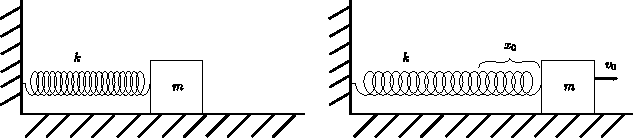
\includegraphics{figures/springsystem2.pdf}
\end{figure}
Þá er gormurinn á einfaldri sveifluhreyfingu um jafnvægisstöðu sína og hreyfilýsing gormsins er
\begin{align*}
    x(t) = x_0 \cos(\omega t) + \frac{v_0}{\omega} \sin(\omega t).
\end{align*}
Þar sem $\omega = \sqrt{\frac{k}{m}}$ er sveiflutíðni gormsins. Sveiflutími gormsins er gefinn með $T = \frac{2\pi}{\omega} = 2\pi \sqrt{\frac{m}{k}}$.
\end{theorem}
\end{tcolorbox}

\begin{minipage}{\linewidth}

\begin{wrapfigure}{r}{1.8in}
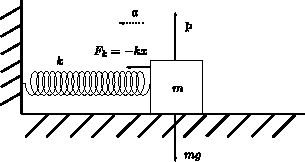
\includegraphics[width=2.2in]{figures/forces-spring.pdf}
\end{wrapfigure}

\textbf{Útleiðsla} Skoðum kraftamynd fyrir kubbinn. Gormkrafturinn er alltaf í gagnstæða stefnu miðað við strekkingu/þjöppun gormsins svo við höfum að:
\begin{align*}
    ma = -kx \implies m\Ddot{x} = -kx \implies \Ddot{x} = - \frac{k}{m}x.
\end{align*}
Svo að gormurinn er á einfaldri sveifluhreyfingu með horntíðni $\omega = \sqrt{\frac{k}{m}}$. Samkvæmt reglu \ref{regla:einfold-sveifla} má því finna fasta $A, B \in \R$ þannig að:
\end{minipage}
\begin{align*}
    x(t) = A\cos(\omega t) + B\sin(\omega t)
\end{align*}
Við athugum að upphafsskilyrðið $x(0) = x_0$ gefur að:
\begin{align*}
    x_0 = x(0) = A \cos(\omega \cdot 0) + B \sin(\omega \cdot 0) = A \cdot 1  + B \cdot 0 = A.
\end{align*}
Athugum síðan að með því að diffra $x(t)$ höfum við að:
\begin{align*}
   v(t) = \dot{x}(t) = -A\omega \sin(\omega t) + B\omega \cos(\omega t)
\end{align*}
Upphafsskilyrðið $v(0) = v_0$ gefur þá að:
\begin{align*}
    v_0 = v(0) = -A\omega \sin(\omega \cdot 0) + B\omega \cos(\omega \cdot 0) = -A \omega \cdot 0 + B \omega \cdot 1 = B\omega \implies B = \frac{v_0}{\omega}.
\end{align*}
En þar með höfum við sýnt að hreyfilýsing gormsins sé gefin með:
\begin{align*}
    x(t) = A\cos(\omega t) + B\sin(\omega t) = x_0 \cos(\omega t) + \frac{v_0}{\omega} \sin(\omega t).
\end{align*}
Að lokum athugum við að lotutími sveiflunnar er þá fundin með því að athuga að:
\begin{align*}
    \omega T = 2\pi \implies T = \frac{2\pi}{\omega} = 2\pi \sqrt{\frac{m}{k}}.
\end{align*}
Sem er þá tíminn sem líður frá því að gorminum er sleppt og þar til hann er aftur á sama stað.
\qed


\begin{tcolorbox}
\begin{theorem}
Hreyfilýsingu gormsins í lögmáli \ref{law:springs} má einnig rita á eftirfarandi formi:
\begin{align*}
    x(t) = A\cos(\omega t + \varphi)
\end{align*}
Þar sem $A, \varphi \in \R$ eru fastar sem ákvarðast af upphafsskilyrðunum $x(0) = x_0$ og $v(0) = \dot{x}(0) = v_0$.
\end{theorem}
\end{tcolorbox}

\textbf{Útleiðsla:} Þetta leiðir beint af Hornafallahaxi Arnars (regla \ref{regla:hornafallahaxArnars}). Talan $A$ kallast þá \textbf{útslag} gormsins og talan $\varphi$ kallast \textbf{fasahorn}. Við sjáum reyndar með samanburði við hornafallahax Arnars að þá er:
\begin{align*}
    A = \sqrt{x_0^2 + \left(\frac{v_0}{\omega}\right)^2}, \hspace{1cm} \varphi = -\arctan(\frac{v_0}{x_0\omega})
\end{align*}
\qed

\vspace{0.2cm}

\begin{tcolorbox}
\begin{theorem}
Orkan er varðveitt fyrir gormhreyfinguna í lögmáli \ref{law:springs}.
\end{theorem}
\end{tcolorbox}
\textbf{Útleiðsla:} Athugum fyrst að ef $x(t) = A\cos(\omega t + \varphi)$ þá er $\dot{x}(t) = -A\omega \sin(\omega t + \varphi)$. Höfum að:
\begin{align*}
    E(t) &= \frac{1}{2}m\dot{x}^2 + \frac{1}{2}kx^2 \\
    &= \frac{1}{2}m \left( -A\omega \sin(\omega t + \varphi)\right)^2  + \frac{1}{2}k\left(A \cos(\omega t + \varphi) \right)^2 \\
    &= \frac{1}{2}m \omega^2 A^2 \sin^2(\omega t + \varphi) + \frac{1}{2}k A^2\cos^2(\omega t + \varphi) \\
    &= \frac{1}{2}kA^2.
\end{align*}
Þar sem við höfum notað að $\omega^2 = \frac{k}{m}$ ásamt reglu Pýþagórasar $\sin^2\theta + \cos^2\theta = 1$.
\qed


\begin{comment}
\begin{align*}
    E(t) &= \frac{1}{2}m\dot{x}^2 + \frac{1}{2}kx^2 \\
    &= \frac{1}{2}m \left( -x_0\omega \sin(\omega t) + v_0 \cos(\omega t) \right)^2 + \frac{1}{2}k \left(  x_0\cos(\omega t) + \frac{v_0}{\omega}\sin(\omega t) \right)^2 \\
    &= \frac{1}{2}m \left( x_0^2\omega^2 \sin^2(\omega t) - 2x_0\omega v_0 \sin(\omega t)\cos(\omega t) + v_0^2 \cos^2(\omega t) \right) \\ &\hspace{3cm} + \frac{1}{2}k\left( x_0^2 \cos^2(\omega t) + \frac{2x_0v_0}{\omega}\cos(\omega t) \sin(\omega t) + \frac{v_0^2}{\omega^2}\sin^2(\omega t) \right) \\
    &= \frac{1}{2}kx_0^2 + \frac{1}{2}mv_0^2 \\ 
    &=  E(0).
\end{align*}
\end{comment}

\vspace{0.3cm}

\section{Lóðréttur gormur}

En hvað ef við festum gorminn okkar lóðrétt við loft og hengjum síðan massa neðan á gorminn? Þá mun gormurinn fá nýja jafnvægisstöðu, $y_0$, sem við getum fundið með því að athuga að þá er:
\begin{align*}
    mg = ky_0 \implies y_0 = \frac{mg}{k}.
\end{align*}
Hugsum okkur síðan að við strekkjum gorminn út um eitthvað $y$ (miðað við nýju jafnvægisstöðu gormsins). Þá mun gormurinn sveiflast um nýju jafnvægisstöðuna sína $y_0$ með sveiflutíðni $\omega = \sqrt{\frac{k}{m}}$. Við höfum nefnilega að kraftajafnan verður:
\begin{align*}
    ma = -k(y+y_0) + mg \implies \Ddot{y} =  -\frac{k}{m}y + g - \frac{k}{m}y_0 = -\frac{k}{m}y
\end{align*}
Þar sem við höfum notað að $y_0 = \frac{mg}{k}$. En þar með sjáum við að aftur er gormurinn á einfaldri sveifluhreyfingu (um nýju jafnvægisstöðu gormsins) með sveiflutíðni $\omega = \sqrt{\frac{k}{m}}$ og hreyfilýsingin er gefin með:
\begin{align*}
    y(t) = A \cos(\omega t + \varphi)
\end{align*}
þar sem $A$ og $\varphi$ eru fastar sem ákvarðast út frá upphafsskilirðunum $y(0)$ og $v(0) = \dot{y}(0)$. Við getum líka sýnt að orkan er varðveitt í lóðréttum sveiflum. Höfum að:
\begin{align*}
    E(t) &= \frac{1}{2}m\dot{y}^2 + \frac{1}{2}k(y + y_0)^2 - mg(y+y_0) \\
    &= \frac{1}{2}kA^2 + ky_0y + \frac{1}{2}ky_0^2 - mgy - mgy_0 \\
    &= \frac{1}{2}kA^2 - \frac{1}{2}mgy_0.
\end{align*}


\section{Pendúll}

\begin{tcolorbox}
\begin{theorem} \label{law:pendulum}
Lítum á pendúl sem samastendur af massa $m$ sem hangir í massalausu bandi af lengd $\ell$. Hugsum okkur að við drögum massann út þannig að upphafshornið sem bandið myndar við lóðrétt sé $\theta_0$ og hugsum okkur að við sleppum massanum með upphafshornhraða $\omega_0$.
\begin{figure}[H]
    \centering
    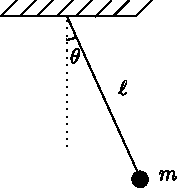
\includegraphics{figures/pendulum.pdf}
\end{figure}
Þá er pendúllinn á einfaldri sveifluhreyfingu um jafnvægisstöðu sína og hreyfilýsing pendúlsins er
\begin{align*}
    \theta(t) = \theta_0 \cos(\omega t) + \frac{\omega_0}{\omega}\sin(\omega t)
\end{align*}
Þar sem $\omega = \sqrt{\frac{g}{\ell}}$ er sveiflutíðni pendúlsins. Sveiflutími pendúlsins er gefinn með $T = \frac{2\pi}{\omega} = 2\pi \sqrt{\frac{\ell}{g}}$.
\end{theorem}
\end{tcolorbox}

\begin{minipage}{\linewidth}

\begin{wrapfigure}{r}{1.5in}
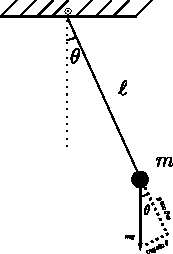
\includegraphics[scale = 1.25]{figures/pendulum-2.pdf}
\end{wrapfigure}

\textbf{Útleiðsla} Skoðum kraftamynd fyrir pendúlinn. Skrifum niður kraftvægisjöfnu um snúningsás pendúlsins (veljum snúningsásinn út úr blaðinu því þá er $\theta$ jákvætt í snúningsstefnuna). Við höfum þá að kraftvægisjafnan verður:
\begin{align*}
    \tau_{\text{heild}} = \tau_{m} \implies I\alpha = -mg\ell \sin\theta
\end{align*}
Notum síðan að $\alpha = \Ddot{\theta}$ og notum nálgunina að $\sin\theta \approx \theta$ fyrir lítil horn. Þá höfum við að kraftvægisjafnan verður:
\begin{align*}
    I\Ddot{\theta} = -mg\ell \sin\theta \approx -mg\ell \theta
\end{align*}
En hverfitregða massans $m$ um snúningsásinn er $I_m = m\ell^2$ svo við ályktum að:
\begin{align*}
    m\ell^2 \Ddot{\theta} = -mg\ell\theta \implies \Ddot{\theta} = -\frac{g}{\ell}\theta
\end{align*}
Svo að pendúllinn er á einfaldri sveifluhreyfingu með horntíðni $\omega = \sqrt{\frac{g}{\ell}}$. Samkvæmt reglu \ref{regla:einfold-sveifla} má því finna fasta $A, B \in \R$ þannig að:
\end{minipage}
\begin{align*}
    \theta(t) = A\cos(\omega t) + B\sin(\omega t)
\end{align*}
Upphafsskilyrðið $\theta(t) = \theta_0$ gefur þá að $A = \theta_0$ og við athugum að $\dot{\theta}(t) = -A\omega \sin(\omega t) + B\omega \cos(\omega t)$ svo við ályktum að upphafsskilyrðið $\dot{\theta}(0) = \omega_0$ gefur að $B = \frac{\omega_0}{\omega}$.

\qed

\begin{tcolorbox}
\begin{theorem}
Lítum á pendúl sem samastendur af massa $m$ sem hangir í massalausu bandi af lengd $\ell$. Þá er hreyfilýsing pendúlsins gefin með
\begin{align*}
    \theta(t) = A \cos(\sqrt{\frac{g}{\ell}}t + \varphi)
\end{align*}
Þar sem $A, \varphi \in \R$ ákvarðast af upphafsskilyrðunum $\theta(0) = \theta_0$ og $\dot{\theta}(0) = \omega_0$.
\end{theorem}
\end{tcolorbox}
Reyndar höfum við að $A = \sqrt{\theta_0^2 + \left(\frac{\omega_0}{\omega}\right)^2}$ og $\varphi = -\arctan(\frac{\omega_0}{\theta_0 \omega})$ samkvæmt hornafallahaxi Arnars.

\section{Flókin sveifluhreyfing (ítarefni)}

Nú þegar við höfum talað aðeins um einfalda sveifluhreyfingu getum við talað aðeins um flókna sveifluhreyfingu. Fyrir flókna sveifluhreyfingu bætum við loftmótsstöðu inn í líkanið okkar (núningnum er síðan afar sambærilega bætt við). En loftmótstaðan er háð hraða hlutarins og loftmótstöðukraftinum má lýsa með $F_L = -\beta v$ þar sem $v$ er hraði hlutarins og $\beta$ er fasti sem er háður eðlismassa hlutarins, þverskurðarflatarmáli og eðlismassa flæðiefnisins sem hluturinn hreyfist í (í þessu tilviki loft). Kraftajafnan okkar verður þá fyrir gorminn:
\begin{align*}
    ma = -\beta v - kx \implies m\Ddot{x} = -\beta \dot{x} - kx
\end{align*}
Sem við getum þá umritað á eftirfarandi form:
\begin{align*}
    \Ddot{x} = - \frac{\beta}{m}\dot{x} - \frac{k}{m}x = -2\gamma \dot{x} - \omega^2 x
\end{align*}
þar sem við höfum skilgreint dempunarfastann $\gamma = \frac{\beta}{2m}$ og sveiflutíðnina $\omega = \sqrt{\frac{k}{m}}$. En lausn diffurjöfnunnar hér að ofan er þá gefin með:
\begin{center}
\begin{tcbox}[nobeforeafter]{$x(t) = Ae^{-\gamma t} \cos(\Omega t + \phi).$}
\end{tcbox}
\end{center}
Þar sem $\Omega = \sqrt{\omega^2 - \gamma^2}$ og $A, \phi$ eru fastar sem ákvarðast af upphafsskilyrðunum. Við getum sannað að svo sé með því að diffra ágiskunina okkar:
\begin{align*}
    v(t) = \dot{x}(t) = -A\gamma e^{-\gamma t}\cos(\Omega t + \phi) - A\Omega e^{-\gamma t}\sin(\Omega t + \phi)
\end{align*}
\begin{align*}
    a(t) = \ddot{x}(t) = A\gamma^2 e^{-\gamma t}\cos(\Omega t + \phi) + 2A\gamma \Omega e^{-\gamma t}\sin(\Omega t + \phi) - A\Omega^2 e^{-\gamma t}\cos(\Omega t + \phi)
\end{align*}
En þar með höfum við einmitt að:
\begin{align*}
    -2\gamma \dot{x} - \omega^2 x &= Ae^{-\gamma t} \left( \left( 2\gamma^2  -\omega^2 \right)\cos(\Omega t + \phi) + 2\gamma \Omega \sin(\Omega t + \phi) \right) \\
    &= Ae^{-\gamma t} \left( \left( \gamma^2  -\Omega^2 \right)\cos(\Omega t + \phi) + 2\gamma \Omega \sin(\Omega t + \phi) \right) = \ddot{x}.
\end{align*}
En það sýnir að $x(t) = Ae^{-\gamma t}\cos(\Omega t + \varphi)$ sé lausn á diffurjöfnunni $\ddot{x} = -2\gamma \dot{x} + \omega^2 x$. En það er önnur leið til þess að líta á þetta. Við getum hugsað okkur að $\cos(\Omega t + \phi)$ lýsi sveifluhreyfingu gormsins en að útslagið sé að dempast með tíma samkvæmt $A(t) = A_0 e^{-\gamma t}$ þar sem $A_0$ er útslagið í upphafi við tímann $t = 0$. En þá höfum við að orka kerfisins minnkar sem fall af tíma samkvæmt:
\begin{align*}
    E(t) &= \frac{1}{2}m\dot{x}^2 + \frac{1}{2}kx^2 \\ &= \frac{1}{2}m A_0^2 e^{-2\gamma t}\left( \gamma \cos(\Omega t + \phi) + \Omega \sin(\Omega t + \phi) \right)^2 + \frac{1}{2}kA_0^2 e^{-2\gamma t} \cos^2(\Omega t + \phi) \\
    &= \frac{1}{2}kA_0^2e^{-2\gamma t} + \frac{\gamma^2}{\omega^2}e^{-2\gamma t}\cos(2\Omega t + 2\phi) + \frac{\gamma \Omega}{\omega^2}e^{-2\gamma t}\sin(2\Omega t + 2\phi) \\
    &= \frac{1}{2}kA_0^2 e^{-2\gamma t} + \frac{\gamma}{\omega}e^{-2\gamma t} \cos(2\Omega t + \varphi)
\end{align*}
\begin{minipage}{\linewidth}

\begin{wrapfigure}{r}{1.5in}
\vspace{-1cm}
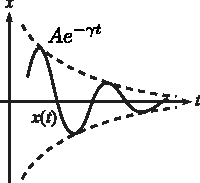
\includegraphics[width = 1.5in]{images/orkan.pdf}
\caption{Hreyfilýsing þar sem útslagið hrörnar.}
\end{wrapfigure}
þar sem við höfum skilgreint $\varphi = 2\phi + \arctan(1-\frac{\omega^2}{\gamma^2})$.

Ef við gerum síðan þá nálgun (án réttlætingar) að $kA_0^2 \gg \frac{\gamma}{\omega}$ þá sjáum við að:
\begin{center} \hspace{-1.5cm}
\begin{tcbox}[nobeforeafter]{$ E(t) \approx \frac{1}{2}kA_0^2e^{-2\gamma t}.$}
\end{tcbox}
\end{center}
En þar með höfum við sýnt að bæði útslag og orka í flókinni sveifluhreyfingu deyr smátt og smátt út með vísishrörnun.
\end{minipage}


\newpage

\section{Dæmi}


\begin{enumerate}[label = \textbf{Dæmi \thechapter.\arabic*.}]

\subsection*{Gormar}

\item \textit{(RK 15.1.)} Vagn með massa $m = \SI{0.82}{kg}$ er festur við gorm með gormstuðul $k = \SI{35}{N/m}$ í verklegu tilraunastofunni. Vagninn getur runnið meðfram láréttum fleti og eftir að við strekkjum á gorminum þá sveiflast vagninn á milli $\SI{20}{cm}$ og $\SI{70}{cm}$ á brautinni.
\begin{enumerate*}[label = \textbf{(\alph*)}]
    \item Hver er sveiflutíðni sveiflunnar? \item Hver er sveiflutími massans? \item Hvert er útslag gormsins? \item Hver er mesti hraði vagnsins á sveifluhreyfingunni? \item Hver er mesta hröðun vagnsins á sveifluhreyfingunni?
\end{enumerate*}

\item \textit{(RK 15.4.)} Hlutur á einfaldri sveifluhreyfingu hefur sveiflutíma $\SI{1.82}{s}$ og útslag $\SI{20}{cm}$. Hversu langan tíma tekur það hlutinn að fara frá jafnvægisstöðu sinni í $x = \SI{0}{cm}$ og í $x = \SI{5}{cm}$?

\vspace{0.1cm}

\begin{minipage}{\linewidth}

\begin{wrapfigure}{r}{1.5in}
\vspace{-0.75cm}
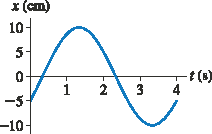
\includegraphics[width = 1.5in]{figures/stada-timi-graf3.pdf}
\end{wrapfigure}

\item \textit{(RK 15.5.)} Lítum á myndina hér til hægri. Á myndinni má sjá stöðu-tíma graf af hlut á einfaldri sveifluhreyfingu. Ákvarðið: \begin{enumerate*}[label = \textbf{(\alph*)}]
    \item Hvert er útslag sveiflunnar?
    \item Hver er sveiflutíminn?
    \item Hver er sveiflutíðnin?
    \item Hvert er fasahornið?
    \item Hver er hreyfilýsing hlutarins?
    \item Hver er hámarkshraði hlutarins, $v_{\text{max}}$?
    \item Hver er hámarkshröðun hlutarins, $a_{\text{max}}$?
\end{enumerate*}
\end{minipage}

\vspace{0.1cm}

\item \textit{(RK 15.16.)} Massi $m = \SI{200}{g}$ er festur við gorm með gormstuðul $k = \SI{32}{N/m}$. Við tímann $t = 0$ er massinn staddur í $x = \SI{5.0}{cm}$ og hefur hraðann $v_x = \SI{-30}{cm/s}$. Ákvarðið \begin{enumerate*}[label = \textbf{(\alph*)}]
    \item Sveiflutíðnina
    \item Sveiflutímann
    \item Hreyfilýsinguna
    \item Mesta útslagið
    \item Mesta hraðann
    \item Mestu hröðunina.
\end{enumerate*}

\item \textit{(RK 15.19.)} Nemandi nokkur er að hoppa á trampólíni. Í hæsta punkti eru fætur hans $\SI{55}{cm}$ fyrir ofan trampólínið en í lægstu stöðu sígur trampólíndúkurinn niður um $\SI{15}{cm}$ áður en nemandinn skýst aftur upp. Í hversu langan tíma er nemandinn í snertingu við trampólínið?

\begin{comment}
\item \textit{(RK 15.21.)} Massi $m = \SI{500}{g}$ er festur í gorm sem hangir í lóðréttri stöðu. Gormurinn sígur þá niður í nýja jafnvægisstöðu sem er $\SI{20}{cm}$ fyrir neðan upphaflegu jafnvægisstöðu gormsins. Hver er gormstuðull gormsins? Nú er gormurinn dreginn út um vegalengd $\SI{10}{cm}$ frá nýju jafnvægisstöðunni og sleppt. Hver verður hreyfilýsing massans í sveifluhreyfingunni?
\end{comment}

\begin{comment}

\item \textit{(RK 15.53.)} Kassi með massa $M = \SI{1.00}{kg}$ stendur á núningslausum, láréttum fleti og er festur við gorm með gormstuðul $k = \SI{2500}{N/m}$. Byssukúlu með massa $m = \SI{10}{g}$ er nú skotið inn í kassann þannig að byssukúlan festist inni í kassanum. Þá byrjar kassinn (og byssukúlan) að sveiflast um jafnvægisstöðu sína þannig að mesta útslag sveifluhreyfingarinnar er $\SI{10.0}{cm}$. Hver var upphafshraði byssukúlunnar? Hver er sveiflutíminn?

\end{comment}

\item \textbf{(Vorpróf 2016)} Einfaldri sveifluhreyfingu er lýst með jöfnunni $x(t) = \SI{0.35}{} \cos(\SI{15.0}{} t + \SI{0.60}{})$ þar sem allar stærðir eru í SI-einingum og horn mæld í radíönum. \begin{enumerate*}[label = \textbf{(\alph*)}]
    \item Finnið mesta hraða í sveiflunni. Við hvaða gildi á $x$ er hraðinn mestur?
    \item Hver er mesta hröðunin í sveiflunni? Við hvaða gildi á $x$ verður hröðunin mest?
\end{enumerate*}

\item \textbf{(Vorpróf 2017)} Staðsetningu $\SI{0.650}{kg}$ massa á einfaldri sveifluhreyfingu sem festur er við gorm með gormstuðul $k$ má lýsa með jöfnunni $x(t) = \SI{0.25}{} \sin(\SI{4.70}{}\cdot t)$ þar sem allar stærðir eru í SI-einingum og horn í radíönum. \begin{enumerate*}[label = \textbf{(\alph*)}]
    \item Hvert er útslag sveifluhreyfingarinnar?
    \item Hver er sveiflutíðnin?
    \item Hver er sveiflutíminn?
    \item Hver er heildarorka massans?
    \item Hver er hreyfiorka massans þegar $x = \SI{15}{cm}$?
\end{enumerate*}

\item \textbf{(Vorpróf 2019)} Kubbur með massa $\SI{400}{g}$ hvílir á núningslausum láréttum fleti. Hann er festur við gorm með gormstuðul $k = \SI{62}{N/m}$ og dreginn út um vegalengd $\SI{12}{cm}$ frá jafnvægisstöðu gormsins. Kubbnum er sleppt úr kyrrstöðu þannig að hann byrjar að sveiflast með einfaldri sveifluhreyfingu um jafnvægisstöðu sína. \begin{enumerate*}[label = \textbf{(\alph*)}]
    \item Finnið sveiflutíma kubbsins.
    \item Finnið hreyfilýsingu kubbsins, það er, finnið staðsetningu hans, $x(t)$, sem fall af tíma.
    \item Við hvaða tíma er hraði kubbsins mestur?
    \item Hver er mesta hröðunin sem kubburinn verður fyrir á sveifluhreyfingunni?
\end{enumerate*}

\begin{comment}

\begin{minipage}{\linewidth}

\begin{wrapfigure}{r}{2in}
\vspace{-1.2cm}
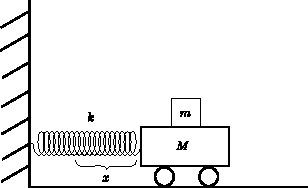
\includegraphics[width = 2.4in]{figures/kubb-spring-kubb.pdf}
\end{wrapfigure}

\item \textit{(RK 15.52.)} Vagn með massa $M$ stendur á núningslausum, láréttum fleti. Vagninn er festur við gorm með gormstuðul $k$. Ofan á vagninum stendur kassi með massa $m$. Þegar við rétt svo ýtum við vagninum þá sveiflast vagninn um jafnvægisstöðu sína með sveiflutíma $T = \SI{1.5}{s}$. Mesta útslagið sem kerfið þolir án þess að kassinn byrji að renna til er $A = \SI{40}{cm}$. Hver er núningsstuðullinn milli kassans og vagnsins?
\end{minipage}
\end{comment}

\vspace{0.1cm}

\begin{minipage}{\linewidth}

\begin{wrapfigure}{r}{1.5in}
\vspace{-0.5cm}
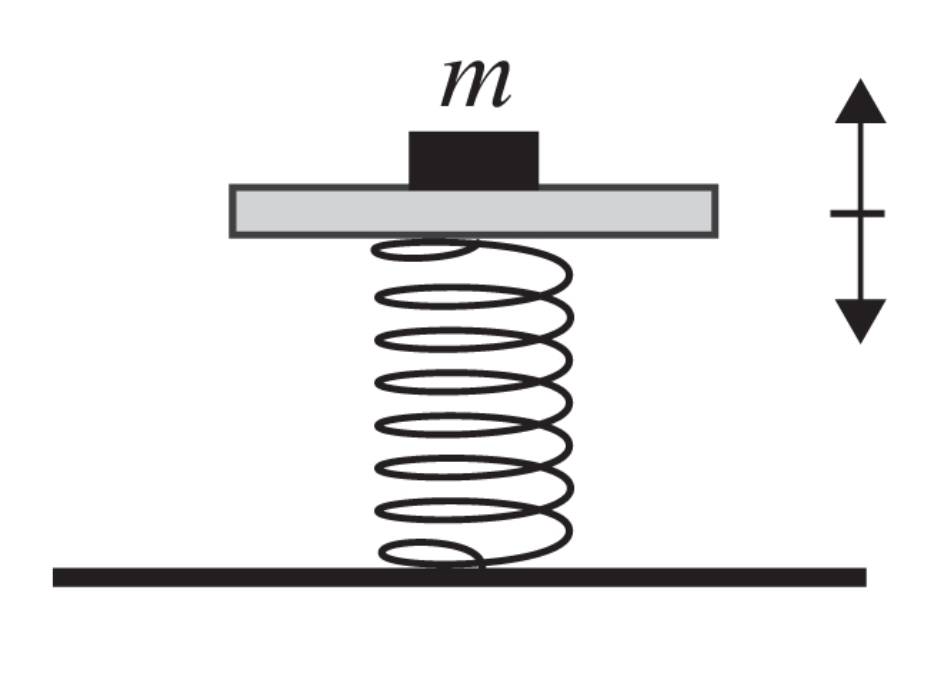
\includegraphics[width = 1.5in]{images/vorprof2013.png}
\end{wrapfigure}

\item \textbf{(Vorpróf 2013)} Myndin hér til hægri sýnir sveiflukerfi sem samanstendur af gormi með áfastri láréttri plötu. Platan er á lóðréttri sveifluhreyfingu með $\SI{6.0}{cm}$ sveifluvídd og sveiflutíma $\SI{0.80}{s}$. Ofan á plötunni liggur hlutur með massann $m = \SI{100}{g}$.
\begin{enumerate*}[label = \textbf{(\alph*)}]
    \item Hver er hröðun plötunnar í neðstu stöðu sveiflunnar?
    \item Með hversu stórum krafti þrýstir platan á hlutinn í neðstu stöðu sveiflunnar?
\end{enumerate*}
\end{minipage}

\vspace{0.2cm}

\item \textit{(RK 15.48.)} Hugrakkur nemandi með massa $\SI{75}{kg}$ stekkur fram af brú með $\SI{12}{m}$ langri (massalausri) teygju sem er fest við fætur nemandans. Líta má á teygjuna sem gorm með gormstuðull $\SI{430}{N/m}$.
\begin{enumerate*}[label = \textbf{(\alph*)}]
    \item Hversu langt fyrir neðan brúnna verður lægsti punkturinn sem nemandinn nær í stökkinu?
    \item Hver er hröðun nemandans í lægsta punkti stökksins?
    \item Hversu langan tíma tekur það nemandan að ná þessum lægsta punkti?
\end{enumerate*}



\begin{comment}

\vspace{0.1cm}

\begin{minipage}{\linewidth}

\begin{wrapfigure}{r}{2in}
\vspace{-1.2cm}
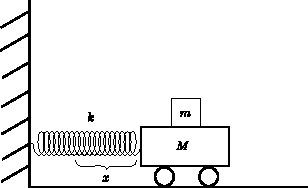
\includegraphics[width = 2.4in]{figures/kubb-spring-kubb.pdf}
\end{wrapfigure}

\item \textit{(RK 15.52.)} Vagn með massa $M$ stendur á núningslausum, láréttum fleti. Vagninn er festur við gorm með gormstuðul $k$. Ofan á vagninum stendur kassi með massa $m$. Þegar við rétt svo ýtum við vagninum þá sveiflast vagninn um jafnvægisstöðu sína með sveiflutíma $T = \SI{1.5}{s}$. Mesta útslagið sem kerfið þolir án þess að kassinn byrji að renna til er $A = \SI{40}{cm}$. Hver er núningsstuðullinn milli kassans og vagnsins?
\end{minipage}

\vspace{0.5cm}

\item \textit{(RK 15.53.)} Kassi með massa $M = \SI{1.00}{kg}$ stendur á núningslausum, láréttum fleti og er festur við gorm með gormstuðul $k = \SI{2500}{N/m}$. Byssukúlu með massa $m = \SI{10}{g}$ er nú skotið inn í kassann þannig að byssukúlan festist inni í kassanum. Þá byrjar kassinn (og byssukúlan) að sveiflast um jafnvægisstöðu sína þannig að mesta útslag sveifluhreyfingarinnar er $\SI{10.0}{cm}$. Hver var upphafshraði byssukúlunnar?

\end{comment}

\newpage

\subsection*{Hreyfilýsing pendúls}

\item \textit{(RK 15.28.)} Festum massa $m = \SI{200}{g}$ á enda $\SI{1.0}{m}$ pendúls. Hver er sveiflutími pendúlsins á Venusi þar sem þyngdarhröðunin er $g_V = \SI{8.87}{m/s^2}$? En á Mars þar sem þyngdarhröðunin er $g_M = \SI{3.71}{m/s^2}$?

\item \textit{(RK 15.30.)} Massi $m = \SI{100}{g}$ er festur í pendúl af lengd $\SI{1.0}{m}$ og sleppt úr kyrrstöðu þegar pendúllinn myndar horn $\theta_0 = \SI{8.0}{\degree}$ miðað við lárétt. Hversu langur tími líður frá því að pendúlnum er sleppt og þar til að hann myndar horn $\theta = \SI{4.0}{\degree}$ miðað við lóðrétt hinum meginn miðað við jafnvægisstöðu pendúlsins?

\item \textit{(RK 15.55.)} Segja má að Galíleó Galíleí hafi fundið upp tímann. Sagan segir að árið 1583 þegar hann var staddur í messu í kaþólsku dómkirkjunni í Pisa þá hafi hann tekið eftir lampa sem sveiflaðist fram og til baka fyrir ofan altarið. Hann tók eftir því að sveiflutími lampans var alltaf sá sami óháð útslagi lampans. Galíleó notaði púlsinn sinn til þess að meta sveiflutímann. Hver er lengd pendúlsins ef Galíleó mælir að $5$ pendúlsveiflur taki um það bil $\SI{37}{hjartslög}$ og hjartað hans slær $\SI{80}{slög/mín}$?



\subsection*{Öðruvísi sveifluhreyfing}

\begin{minipage}{\linewidth}

\begin{wrapfigure}{r}{1.25in}
\vspace{-1cm}
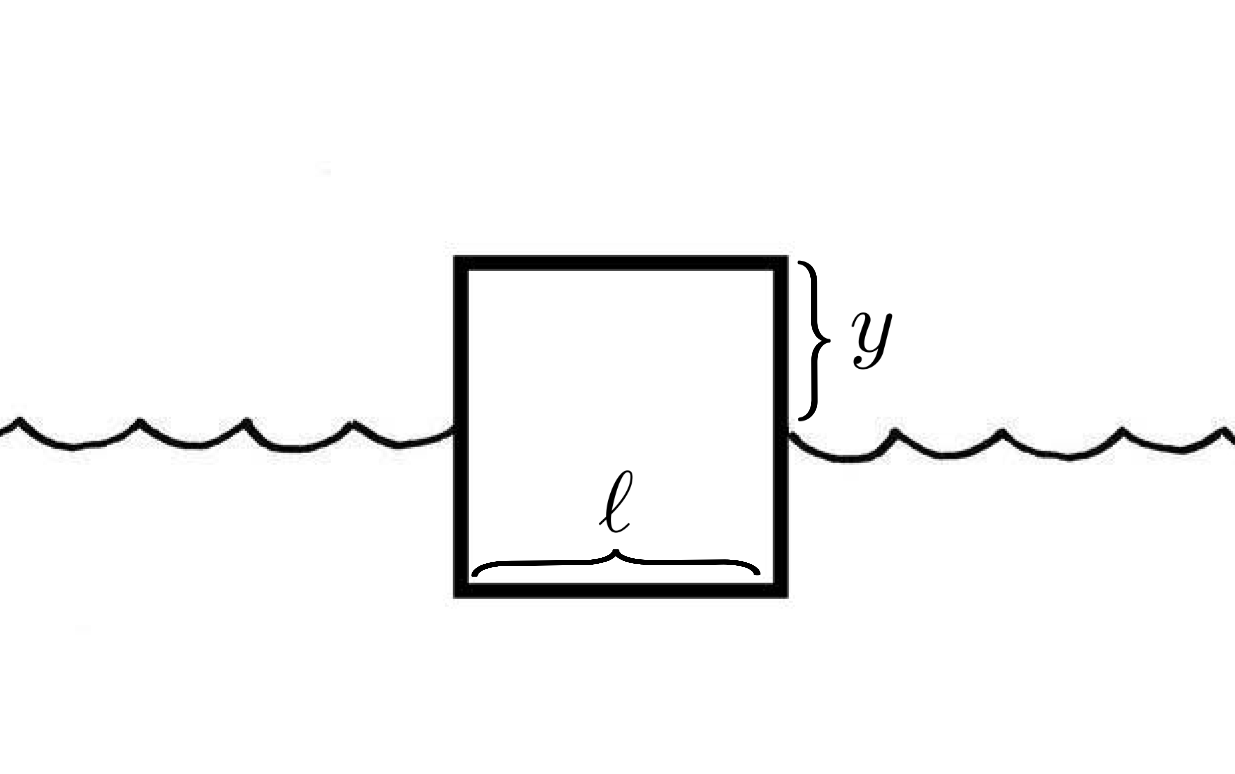
\includegraphics[width=1.8in]{images/kubbursjor.png}
\end{wrapfigure}
\item \textbf{(Vorpróf 2019)} Gegnheill kassi með allar hliðar jafnlangar, $\ell = \SI{0.50}{m}$, og með eðlismassa $\rho_k = \SI{650}{kg/m^3}$ flýtur úti á rúmsjó. Eðlismassi sjávar er gefinn með $\rho_s = \SI{1027}{kg/m^3}$. Fugl með massa $\SI{9.0}{kg}$ sest á kassann svo að yfirborðið lækkar. Þegar fuglinn flýgur af kassanum byrjar kassinn að sveiflast um jafnvægisstöðu sína með einfaldri sveifluhreyfingu. Finnið hreyfilýsingu kassans, $y(t)$.
\end{minipage}

\begin{minipage}{\linewidth}

\begin{wrapfigure}{r}{1in}
\vspace{0.5cm}
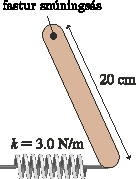
\includegraphics[width=1.25in]{figures/fastur-snunas.pdf}
\end{wrapfigure}

\item \textit{(RK 15.66.)} Hugsum okkur að við ætlum að smíða hax póstlagninarfyrirtæki sem sendir pakka milli Íslands og Ástralíu (hinum meginn á hnettinum). Hugsum okkur að í staðinn fyrir að sigla eða fljúga með pakkana þá ákveðum við að bora göng beint í gegnum miðju jarðarinnar. Hugsum okkur síðan að við hendum pakkanum ofan í göngin. Hunsum eins og alltaf loftmótstöðu og gerum ráð fyrir því að jörðin hafi einsleitan eðlismassa. Þá mun þyngdarkrafturinn sem pakkinn finnur fyrir breytast eftir því sem hann nálgast miðju jarðarinnar. Reyndar er hægt að sýna að í fjarlægð $r$ frá miðju jarðarinnar þar sem $0 < r < R$ og $R$ er geisli jarðarinnar þá er þyngdarhröðunin gefin með $g(r) = \frac{r}{R}g$ þar sem $g = \SI{9.82}{m/s^2}$ er þyngdarhröðunin við yfirborð jarðarinnar. Hversu langan tíma tæki þá að senda pakka til Ástralíu?

\item \textit{(RK 15.81.)} Hér til hægri sést einsleit stöng af lengd $\ell = \SI{20}{cm}$ með massa $m = \SI{200}{g}$. Stöngin er fest með nagla í efri endan og við gorm með gormstuðul $k = \SI{3.0}{N/m}$ við neðri endann. Þegar stöngin hangir algjörlega lóðrétt þá er gormurinn í jafnvægisstöðu sinni. Nú drögum við stöngina út um horn $\theta_0$ miðað við lárétt og sleppum stönginni úr kyrrstöðu. Hver verður sveiflutíðni stangarinnar?

\end{minipage}

\end{enumerate}


\section*{Svör}

\begin{enumerate*}[label = \vspace{0.15cm} \textbf{(\arabic*)}]
  \item $\omega = \SI{6.53}{rad/s}$, $T = \SI{0.96}{s}$, $A = \SI{25}{cm}$, $v_{\text{max}} = \SI{1.63}{m/s}$, $a_{\text{max}} = \SI{10.7}{m/s^2}$.
  \item $\tau = \SI{73}{ms}$.
  \item $A = \SI{10}{cm}$, $T = \SI{4.0}{s}$, $\omega = \SI{1.57}{rad/s}$, $v_{\text{max}} = \SI{0.16}{m/s}$, $a_{\text{max}} = \SI{0.25}{m/s^2}$.
  \item $\omega = \SI{12.6}{rad/s}$, $T = \SI{0.50}{s}$, $A = \SI{5.5}{cm}$, $v_{\text{max}} = \SI{0.69}{m/s}$, $a_{\text{max}} = \SI{8.7}{m/s^2}$.
  \item $\tau = \SI{0.13}{s}$.
  \item $v_{\text{max}} = \SI{5.3}{m/s}$, $a_{\text{max}} = \SI{79}{m/s^2}$.
  \item $T = \SI{1.34}{s}$, $E = \SI{0.45}{J}$, $K = \SI{0.29}{J}$.
  \item $T = \SI{0.51}{s}$, $\tau = \SI{0.13}{s}$, $a_{\text{max}} = \SI{18.5}{m/s^2}$.
  \item $a_{\text{max}} = \SI{3.74}{m/s^2}$, $Þ = \SI{1.4}{N}$.
  \item $\ell + x = \SI{20.4}{m}$, $a_{\text{max}} = \SI{45.7}{m/s^2}$, $T = \SI{2.34}{s}$.
  \item $\omega_V = \SI{2.98}{rad/s}$, $\omega_M = \SI{1.93}{rad/s}$.
  \item $\tau = \SI{0.67}{s}$.
  \item $\ell = \SI{7.8}{m}$.
  \item $\omega = \sqrt{\frac{\rho_{\text{vökvi}}g}{\rho_{\text{hlutur}}\ell}} = \SI{5.6}{rad/s}$, $A = \SI{3.6}{cm}$.
  \item $T = \SI{42}{mín}$ og $\SI{10}{sek}$. 
  \item $\omega = \sqrt{\frac{3g}{2\ell} + \frac{3k}{m}}$.
\end{enumerate*}

\newpage